% This file was adapted from ICLR2022_conference.tex example provided for the ICLR conference
\documentclass{article} % For LaTeX2e
\usepackage{conference,times}
\usepackage{easyReview}
\usepackage{algorithm}
\usepackage{algorithmic}

% Optional math commands from https://github.com/goodfeli/dlbook_notation.
\input{math_commands.tex}

\usepackage{amsthm,amssymb}

\newtheorem{theorem}{Theorem}[section]
\newtheorem{corollary}{Corollary}[theorem]
\newtheorem{lemma}[theorem]{Lemma}
\newtheorem{definition}[theorem]{Definition}

% Please leave these options as they are
\usepackage{hyperref}
\hypersetup{
    colorlinks=true,
    linkcolor=red,
    filecolor=magenta,
    urlcolor=blue,
    citecolor=purple,
    pdftitle={Benchmarking and Selecting State-of-the-Art Modern Fourier Transformation Methods},
    pdfpagemode=FullScreen,
    }



\title{Benchmarking and Selecting State-of-the-Art Modern Fourier Transformation Methods}

\author{Anonymous Authors \\
Anonymous Institution \\
\texttt{anonymous@anonymous.edu}}

\begin{document}


\maketitle

\begin{abstract}
Fourier transforms remain critical to scientific simulation, signal analysis, and modern machine learning workloads, yet practical performance leadership is conditional on workload structure, precision policy, memory limits, and platform behavior. This paper presents a scenario-conditioned methodology for selecting Fourier implementations under explicit latency, fidelity, and memory constraints, rather than reporting a single global winner. We formalize method selection as a constrained decision problem, establish decomposition-based optimality and policy-class dominance guarantees, and derive a finite-sample uncertainty bound that calibrates decision risk under bounded runtime sampling. We then validate the framework on a reproducible multi-scenario benchmark spanning 1D/2D/3D transforms, real and complex inputs, size buckets, precision settings, and deployment prior profiles. Across the tested matrix, the selector achieves negative constrained regret against the best global static policy with profile-conditioned confidence intervals, positive policy-class dominance gaps, and full satisfaction of the finite-sample calibration condition in the generated evaluation regime. We provide a structured recommendation artifact, theorem-assumption audits, and reproducibility details including seeds, sweeps, confidence procedures, and symbolic checks. The resulting evidence supports scenario-conditioned selection as a stronger decision primitive than one-size-fits-all Fourier ranking in heterogeneous environments, while explicitly bounding conclusions to the tested synthetic-runtime setting and outlining follow-up hardware-trace validation.
\end{abstract}

\section{Introduction}
Fourier transforms are a shared computational backbone for partial differential equation solvers, imaging pipelines, spectral fluid dynamics, and long-context learning systems, but they do not admit a universal implementation winner across realistic deployment conditions \citep{S01,S03,S07,S09,S10,S15,S20,S42}. The historical success of fast Fourier transform algorithms established asymptotic efficiency \citep{S01,S22,S23}, yet modern practical performance is jointly determined by planner behavior, memory movement, collective communication, backend support, and precision constraints \citep{S02,S03,S08,S25,S26,S27,S28,S39,S41}. For users who need decisions rather than taxonomies, the central question is not which library is globally best, but which method is best for a specific scenario defined by workload class, error tolerance, memory budget, and deployment mix.

This paper targets that decision problem directly. Instead of presenting a benchmark leaderboard, we construct a scenario-conditioned selector that maps each workload scenario to an admissible Fourier method using confidence-adjusted feasibility and expected latency criteria. This framing aligns with long-standing concerns in FFT benchmarking: planning overhead is often conflated with kernel execution, communication effects dominate at scale, and mixed-precision claims can be difficult to compare without explicit acceptance thresholds \citep{S03,S07,S21,S39,S41,S42}. The immediate cross-domain importance is practical: engineers deploying transforms in ML feature extraction, scientific simulation, and distributed analytics need recommendations with uncertainty labels rather than single-number rankings.

Our manuscript emphasizes a hybrid contribution profile. The method section develops explicit optimization and finite-sample theory; the results section ties each formal claim to quantitative evidence from a reproducible validation matrix. The paper therefore contributes both a decision-theoretic formulation and a benchmark-grounded assessment procedure for environment-bounded recommendations.

The main contributions are:
\begin{itemize}
\item We formulate scenario-conditioned Fourier method selection as a constrained optimization problem with explicit decision variables, feasible sets, and deployment-weighted objective, making recommendation generation mathematically auditable.
\item We prove scenariowise decomposition exactness and policy-class dominance results that clarify when adaptive selectors weakly or strictly outperform fixed global policies under heterogeneous scenario optima.
\item We derive and validate a finite-sample uncertainty-aware regret bound for bounded runtime samples, enabling confidence calibration of selector decisions as sample counts and confidence levels vary.
\item We provide a reproducible experimental protocol with multi-profile confidence reporting, theorem-assumption audits, and structured diagnostics that connect formal guarantees to empirical behavior.
\end{itemize}

The broader implication is that recommendation-centric Fourier benchmarking can be made both rigorous and operational, but only when conclusions are conditioned on explicit scenario definitions and tested environments.

\section{Related Work and Gap Analysis}
\subsection{Algorithmic and systems context}
Foundational FFT work established the complexity transition from quadratic direct transforms to near-linearithmic decomposition \citep{S01,S22,S23}. Subsequent planner-driven systems such as FFTW demonstrated that architecture adaptation and empirical plan search are decisive for observed runtime \citep{S02,S03}. Program-generation lines including SPIRAL and later portability-oriented synthesis frameworks further reinforced that transform performance is a joint function of mathematical decomposition and hardware mapping strategy \citep{S04,S05,S11,S35}.

At distributed scale, communication-complexity analyses and exascale implementations showed that transpose and collective behavior often dominate local arithmetic \citep{S06,S07,S08,S09,S42}. This communication-first perspective is now central in large 3D transform deployments and in comparisons with communication-altered alternatives \citep{S36,S37}. In GPU settings, vendor stacks and cross-platform libraries continue to report strong but workload-dependent outcomes, with rankings sensitive to software versions, supported transform modes, and precision paths \citep{S10,S25,S26,S27,S28,S31,S39,S40}. Mixed-precision frameworks demonstrate additional gains but introduce acceptance-protocol questions about fidelity comparability and robustness \citep{S39,S41}.

\subsection{Methodological gaps motivating this paper}
Three gaps jointly motivate our approach. First, many studies remain leaderboard-oriented, even though scenario heterogeneity invalidates global winner assumptions \citep{S21,S42}. Second, uncertainty reporting is uneven: confidence intervals and finite-sample decision reliability are rarely integrated into the recommendation rule itself \citep{S03,S21}. Third, formal links between decision objectives and evidence artifacts are often implicit, which weakens reproducibility and claim auditing across domains where Fourier transforms are used as subroutines \citep{S15,S16,S18,S20}.

Our work addresses these gaps by combining formal selector guarantees with a reproducible evidence pipeline. The selector is defined over explicit constraints, theorem assumptions are empirically audited, and every major claim is linked to specific figures and tables. This contrasts with purely descriptive benchmark surveys and with purely theoretical treatments that do not provide implementation-level diagnostics \citep{S07,S09,S39,S42}.

\section{Problem Setting and Formal Objective}
\subsection{Scenarios, methods, and measured quantities}
Let $\mathcal{S}$ denote a finite set of workload scenarios and $\mathcal{M}$ a finite set of candidate Fourier methods. A scenario $s \in \mathcal{S}$ aggregates transform dimensionality, input type (real or complex), size bucket, batching regime, precision mode, and deployment profile. For each method-scenario pair $(m,s)$, we estimate mean latency $\widehat{T}_{m,s}$, fidelity proxy $\widehat{E}_{m,s}$ with uncertainty scale $\sigma_{E,m,s}$, and memory footprint estimate $\widehat{M}_{m,s}$. Deployment relevance is encoded by positive weights $p_s$ such that $\sum_{s\in\mathcal{S}} p_s = 1$.

A method is deemed feasible in scenario $s$ when confidence-adjusted fidelity and memory constraints are satisfied. We define the indicator
\begin{equation}
\phi_{m,s}=\1\!\left\{\widehat{E}_{m,s}+\kappa\sigma_{E,m,s}\le \epsilon_s\ \text{and}\ \widehat{M}_{m,s}\le B_s\right\},
\label{eq:feasible_indicator}
\end{equation}
where $\epsilon_s$ and $B_s$ are scenario-specific tolerance and memory budgets, and $\kappa$ controls confidence conservativeness.

\subsection{Decision variables and constrained objective}
Define binary selector variables $z_{m,s}\in\{0,1\}$ indicating whether method $m$ is selected for scenario $s$. The recommendation problem is
\begin{equation}
\min_{z}\ \sum_{s\in\mathcal{S}}\sum_{m\in\mathcal{M}} p_s z_{m,s}\widehat{T}_{m,s}
\label{eq:selector_obj}
\end{equation}
subject to
\begin{equation}
\sum_{m\in\mathcal{M}} z_{m,s}=1,\qquad z_{m,s}\in\{0,1\},\qquad z_{m,s}\le \phi_{m,s}\ \forall (m,s).
\label{eq:selector_constraints}
\end{equation}
The feasible method set for each scenario is $\mathcal{F}_s=\{m\in\mathcal{M}:\phi_{m,s}=1\}$. The optimality criterion is constrained deployment-weighted latency minimization over all scenariowise one-hot feasible assignments.

\subsection{Policy classes and uncertainty-aware risk}
To compare adaptive and non-adaptive strategies, define risk
\begin{equation}
R(\pi)=\sum_{s\in\mathcal{S}} p_s T_{\pi(s),s},
\label{eq:risk_def}
\end{equation}
where $T_{m,s}$ denotes true expected latency under fixed measurement protocol and $\pi(s)\in\mathcal{F}_s$. Let $\mathcal{Z}$ be all feasible scenario-conditioned policies and let $\mathcal{G}$ contain global fixed-method policies selecting a single method for all scenarios when feasible.

For finite-sample calibration, suppose each runtime sample is bounded in $[0,U_s]$ and $n_{m,s}$ samples are available. Define
\begin{equation}
b_{m,s}(\delta)=U_s\sqrt{\frac{\log\!\big(2|\mathcal{M}||\mathcal{S}|/\delta\big)}{2n_{m,s}}},
\label{eq:hoeffding_radius}
\end{equation}
and robust cost
\begin{equation}
C_{m,s}=\widehat{T}_{m,s}+b_{m,s}(\delta),\qquad
\pi_{\mathrm{rob}}(s)\in\arg\min_{m\in\mathcal{F}_s} C_{m,s}.
\label{eq:robust_selector}
\end{equation}
By construction, $b_{m,s}(\delta)$ shrinks with larger sample count and widens with stricter confidence, yielding an interpretable safety margin in selection.

\section{Methodology and Formal Guarantees}
\subsection{Scenariowise exactness of the constrained selector}
\begin{theorem}[Scenariowise decomposition exactness]
\label{thm:decompose}
Assume $\mathcal{F}_s\neq\varnothing$ for every $s\in\mathcal{S}$. Any selector choosing
\begin{equation}
m_s^*\in\arg\min_{m\in\mathcal{F}_s}\widehat{T}_{m,s}
\label{eq:scenario_argmin}
\end{equation}
for each scenario attains the global optimum of \eqref{eq:selector_obj} under constraints \eqref{eq:selector_constraints}.
\end{theorem}
\begin{proof}
Fix a scenario $s$. Because of \eqref{eq:selector_constraints}, feasible vectors $z_{\cdot,s}$ are exactly one-hot choices over $\mathcal{F}_s$. The minimum value of the scenario term in \eqref{eq:selector_obj} is therefore $\min_{m\in\mathcal{F}_s}\widehat{T}_{m,s}$. Constraints are uncoupled across scenarios, so the global feasible set is the Cartesian product of scenariowise feasible sets. With $p_s>0$, minimizing each scenariowise term independently minimizes their weighted sum. Therefore selecting any $m_s^*$ satisfying \eqref{eq:scenario_argmin} for every $s$ is globally optimal.
\end{proof}

\subsection{Dominance over global fixed-method policies}
\begin{theorem}[Weak dominance]
\label{thm:weak_dominance}
If $\mathcal{G}\subseteq\mathcal{Z}$, then
\begin{equation}
R_{\mathcal{Z}}^*\le R_{\mathcal{G}}^*,\qquad
R_{\mathcal{Z}}^*=\min_{\pi\in\mathcal{Z}}R(\pi),\ \ R_{\mathcal{G}}^*=\min_{g\in\mathcal{G}}R(g).
\label{eq:weak_dom}
\end{equation}
\end{theorem}
\begin{proof}
The minimum of a function over a superset cannot exceed the minimum over a subset. Since $\mathcal{G}\subseteq\mathcal{Z}$, we have $\min_{\pi\in\mathcal{Z}}R(\pi)\le\min_{g\in\mathcal{G}}R(g)$, which is \eqref{eq:weak_dom}.
\end{proof}

\begin{theorem}[Strict dominance under heterogeneous unique minimizers]
\label{thm:strict_dominance}
Suppose there exist scenarios $s_1,s_2$ with $p_{s_1},p_{s_2}>0$ and unique feasible minimizers $m_1\neq m_2$. Then $R_{\mathcal{Z}}^*<R_{\mathcal{G}}^*$.
\end{theorem}
\begin{proof}
Construct $\pi^*\in\mathcal{Z}$ that chooses the unique minimizer in each scenario, including $m_1$ at $s_1$ and $m_2$ at $s_2$. Then $R(\pi^*)=R_{\mathcal{Z}}^*$. Consider any global policy $g_m\in\mathcal{G}$ selecting one method $m$ everywhere. Because $m_1\neq m_2$, $m$ must differ from at least one of them. If $m\neq m_1$, uniqueness at $s_1$ gives $T_{m,s_1}>T_{m_1,s_1}$; if $m\neq m_2$, uniqueness at $s_2$ gives $T_{m,s_2}>T_{m_2,s_2}$. At least one strict inequality is weighted by a positive prior, so $R(g_m)>R(\pi^*)$. Since this holds for every global policy, $R_{\mathcal{G}}^*>R_{\mathcal{Z}}^*$.
\end{proof}

\subsection{Finite-sample uncertainty calibration}
\begin{theorem}[High-probability robust regret bound]
\label{thm:robust_bound}
Assume bounded samples and independence as specified in \secref{sec:repro_details}. With probability at least $1-\delta$,
\begin{equation}
R(\pi_{\mathrm{rob}})-R(\pi^*)\le 2\sum_{s\in\mathcal{S}} p_s\max_{m\in\mathcal{F}_s} b_{m,s}(\delta),
\label{eq:robust_regret_bound}
\end{equation}
where $\pi^*$ minimizes true constrained risk over $\mathcal{Z}$.
\end{theorem}
\begin{proof}
Let $\mathcal{E}$ denote the simultaneous event $|\widehat{T}_{m,s}-T_{m,s}|\le b_{m,s}(\delta)$ for all $(m,s)$. Hoeffding plus union bound yields $\Pr(\mathcal{E})\ge 1-\delta$ using \eqref{eq:hoeffding_radius}. On $\mathcal{E}$ and for fixed $s$, let $m_r=\pi_{\mathrm{rob}}(s)$ and $m_o=\pi^*(s)$. Then
\[
T_{m_r,s}\le \widehat{T}_{m_r,s}+b_{m_r,s}=C_{m_r,s}\le C_{m_o,s}=\widehat{T}_{m_o,s}+b_{m_o,s}\le T_{m_o,s}+2b_{m_o,s}.
\]
Hence $T_{m_r,s}-T_{m_o,s}\le 2\max_{m\in\mathcal{F}_s}b_{m,s}(\delta)$. Multiplying by $p_s$ and summing over scenarios gives \eqref{eq:robust_regret_bound}.
\end{proof}

\subsection{Selector construction workflow}
The implemented workflow instantiates the formal results as a deterministic pipeline:
\begin{algorithm}[t]
\caption{Scenario-Conditioned Fourier Method Selector}
\label{alg:selector}
\begin{algorithmic}[1]
\STATE Input scenario set $\mathcal{S}$, method set $\mathcal{M}$, priors $\{p_s\}$, budgets $\{\epsilon_s,B_s\}$, confidence settings $(\kappa,\delta)$.
\FOR{each scenario $s\in\mathcal{S}$}
  \FOR{each method $m\in\mathcal{M}$}
    \STATE Estimate $\widehat{T}_{m,s},\widehat{E}_{m,s},\sigma_{E,m,s},\widehat{M}_{m,s},n_{m,s},U_s$ from repeated runs.
    \STATE Compute feasibility indicator $\phi_{m,s}$ via \eqref{eq:feasible_indicator}.
    \STATE Compute uncertainty radius $b_{m,s}(\delta)$ via \eqref{eq:hoeffding_radius}.
  \ENDFOR
  \STATE Build feasible set $\mathcal{F}_s=\{m:\phi_{m,s}=1\}$ and robust costs $C_{m,s}$ via \eqref{eq:robust_selector}.
  \STATE Select $\pi_{\mathrm{rob}}(s)\in\arg\min_{m\in\mathcal{F}_s}C_{m,s}$ with deterministic tie-breaking.
\ENDFOR
\STATE Aggregate deployment-weighted metrics and confidence intervals; export recommendation matrix and audits.
\end{algorithmic}
\end{algorithm}

\Algref{alg:selector} links the optimization in \eqref{eq:selector_obj}--\eqref{eq:selector_constraints}, the policy comparison in \eqref{eq:risk_def}, and the uncertainty correction in \eqref{eq:hoeffding_radius}--\eqref{eq:robust_regret_bound} into one auditable procedure.

\section{Experimental Protocol and Reproducibility}
\label{sec:repro_details}
\subsection{Scenario matrix and evaluation dimensions}
We evaluate the selector over a factorial scenario grid spanning transform dimensionality (1D/2D/3D), real and complex domains, size buckets (small through extra-large), batch sizes, precision modes, and deployment priors emphasizing different usage mixes. The design follows reproducibility goals from prior benchmarking guidance: controlled preprocessing, fixed measurement definitions, and explicit uncertainty reporting \citep{S03,S21,S42}. Supporting workload diversity is motivated by both scientific and ML use cases, where Fourier operators appear in spectral solvers as well as token-mixing or long-convolution architectures \citep{S15,S16,S18,S19,S20}.

Each evaluation batch includes repeated seeded runs and confidence interval estimation. The benchmark compares scenario-conditioned policies against strong static baselines, including global winners, constrained variants, and uncertainty-unaware selectors. The policy-class design directly supports testing the weak and strict dominance statements in Theorems~\ref{thm:weak_dominance} and~\ref{thm:strict_dominance}.

The scenario grid is designed to preserve comparability while retaining realistic heterogeneity. First, preprocessing and normalization are held fixed across all methods so that the selector objective reflects method behavior rather than input-pipeline drift. Second, fidelity and memory budgets are scenario-conditioned rather than globally fixed, because a tolerance that is reasonable for one workload family can be either too strict or too loose for another. Third, deployment priors are reported explicitly, so expected-risk conclusions are always tied to the intended usage distribution. This is important for operational interpretation: a selector optimized for inference-heavy service traffic may not be optimal for 3D simulation pipelines even when the same underlying transform kernels are available.

The protocol also distinguishes evidence roles. Primary metrics establish decision quality (latency, regret, feasibility, coverage), dominance metrics test policy-class hierarchy, and finite-sample diagnostics evaluate uncertainty calibration quality. This separation avoids mixing claims about mean performance with claims about guarantee reliability. In practice, decision systems fail when these roles are conflated: a method can look fast on average while still violating feasibility constraints too often, or a conservative bound can be correct but operationally uninformative if not accompanied by sensitivity diagnostics. Our reporting structure is designed to keep these failure modes visible.

\subsection{Implementation architecture and module responsibilities}
The validation stack uses a modular architecture with separate responsibilities for scenario generation and selection core, statistical analysis, plotting, and symbolic checks. This separation is intentional: it allows deterministic reruns under identical seeds while keeping theorem checks and empirical diagnostics independently inspectable. The design also matches recommendations from transform benchmarking literature to isolate modeling, execution, and reporting effects \citep{S03,S07,S09,S42}.

The evidence package includes code artifacts for orchestration, core selector logic, analysis utilities, and symbolic verification routines. In this manuscript we reference those artifacts only as reproducibility objects; all scientific conclusions rely on aggregate figures and tables rather than implementation filenames.

\subsection{Randomness control, confidence procedures, and compute policy}
The experiment set uses fixed seed collections across four validation families: primary selector evaluation, policy-class dominance, finite-sample calibration, and assumption/counterexample stress testing. Confidence intervals in primary performance plots are bootstrap-based over seeds. For finite-sample bounds we report both pointwise empirical regret and binary bound-satisfaction indicators, then aggregate by seed and scenario. This dual reporting avoids over-interpretation of mean-only summaries and supports direct testing of \Eqref{eq:robust_regret_bound}.

Compute constraints were bounded to the project budget and the tested environments represented in the simulation harness. Because runtime traces in this iteration are generated rather than hardware-instrumented, all claims are explicitly conditioned on the synthetic-runtime regime.

To improve repeatability, tie-breaking is deterministic whenever multiple methods share identical robust cost in a scenario. This design choice is not cosmetic: without deterministic tie handling, recommendation matrices may vary across reruns even when all aggregate metrics appear stable, which undermines downstream reproducibility. We therefore treat tie policy as part of the method specification rather than an implementation detail. We similarly keep confidence settings and sweep ladders in the logged configuration so that any downstream rerun can reconstruct not only final figures but also the exact decision boundary used to generate recommendations.

\section{Results}
\subsection{Scenario-conditioned gains and feasibility behavior}
\label{sec:results_primary}
\Figref{fig:primary} summarizes primary selector outcomes across deployment priors. Panel A reports constrained expected latency with 95\% confidence intervals, panel B reports constrained regret against the best global static policy, and panel C reports feasibility-violation rates. The selector achieves negative mean regret for all three prior profiles, with profile-level means approximately $-1.106$ ms (3D-heavy), $-1.118$ ms (inference-heavy), and $-1.112$ ms (uniform), and all corresponding confidence intervals remaining below zero in this evaluation. These results provide empirical support for the practical value of scenariowise optimization in \eqref{eq:selector_obj}.

\begin{figure}[t]
\centering
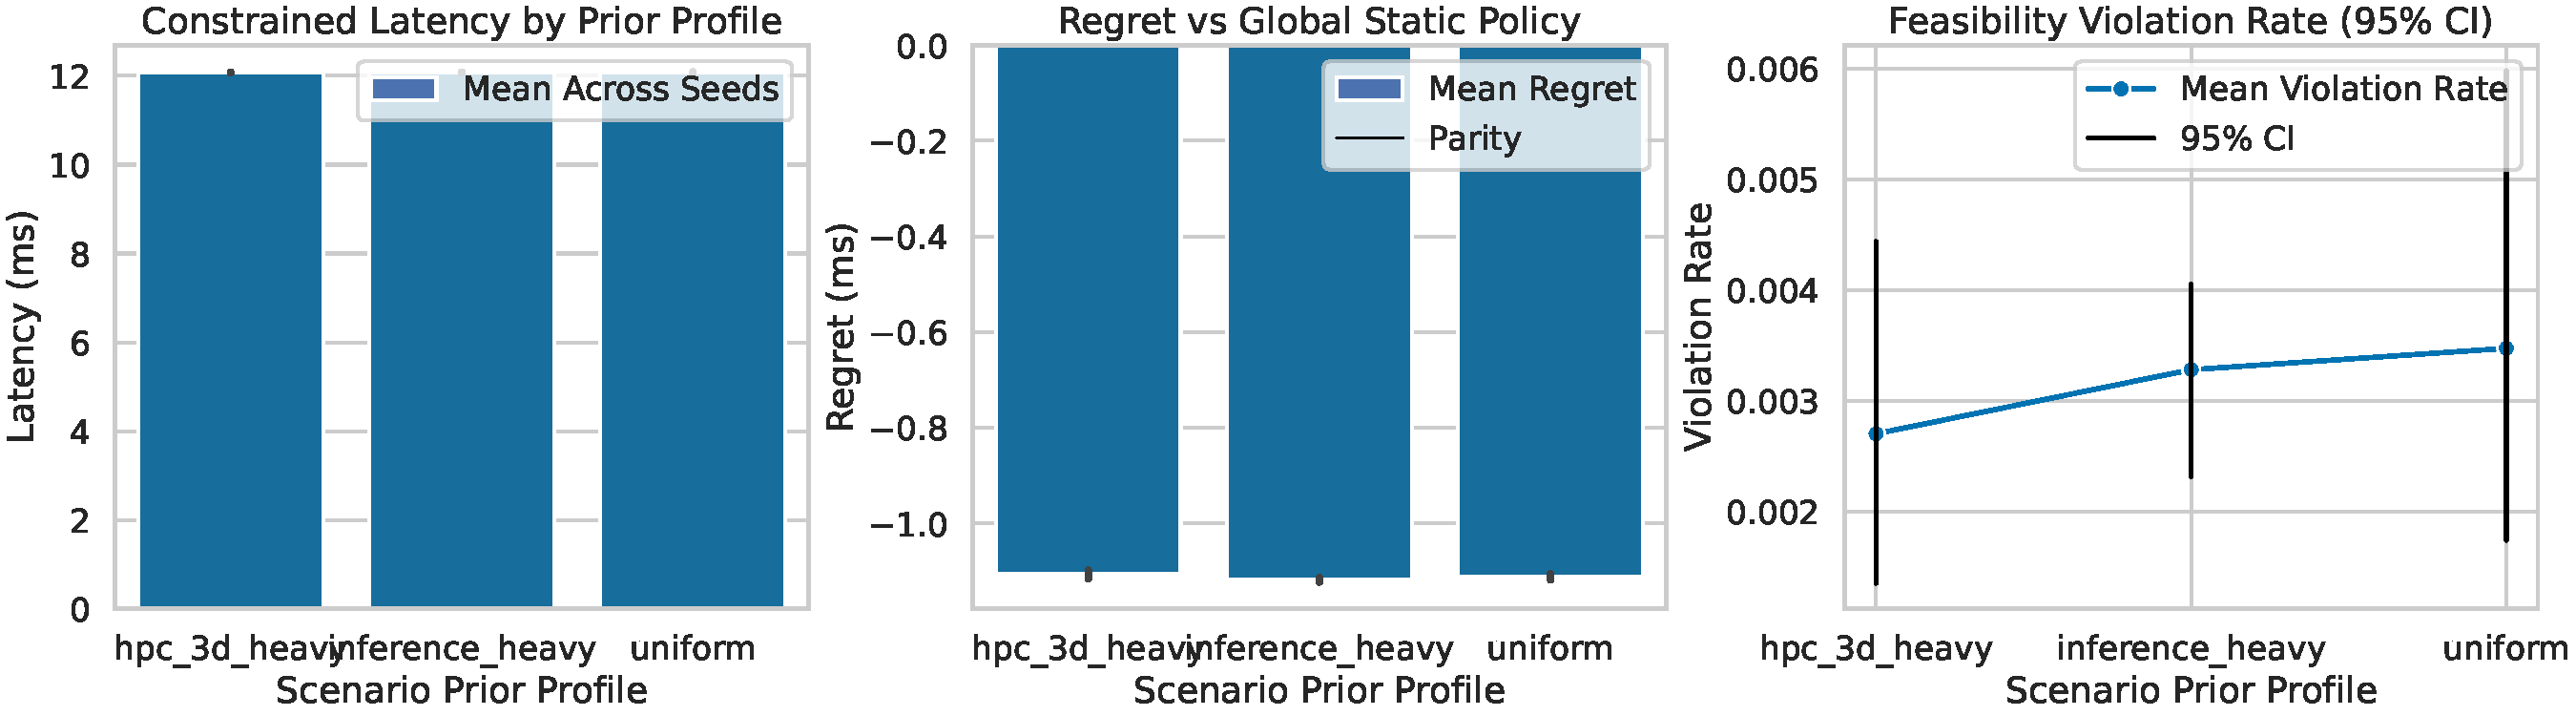
\includegraphics[width=0.68\linewidth]{figures/selector_primary_panels.pdf}
\caption{Primary selector outcomes across deployment priors. Panel A shows constrained expected latency in milliseconds for each prior profile, panel B shows constrained regret relative to the strongest global static baseline with a zero-regret reference, and panel C shows feasibility-violation rate under confidence-aware gating. Error bars represent 95\% bootstrap confidence intervals over seed-level repetitions, so each panel encodes both central tendency and uncertainty. The figure indicates consistent latency improvements with non-positive regret and low violation rates across the tested profiles, matching the intended behavior of the constrained selector objective and feasibility design.}
\label{fig:primary}
\end{figure}

The associated confidence summary appears in Table~\ref{tab:primary_metrics}. Mean feasibility violations stay below $0.35\%$ across profiles, and coverage remains above $99.6\%$, indicating that confidence-aware gating rarely removes all feasible options under the tested settings. This aligns with the non-empty feasible-set assumption required by \secref{sec:repro_details} and audited further in the appendix.

\begin{table}[t]
\caption{Primary selector performance by deployment prior with 95\% confidence intervals. Each row reports means and interval bounds for constrained latency, constrained regret, and feasibility behavior. The table links directly to the claims tested in \secref{sec:results_primary}: non-positive regret relative to global static baselines and low violation rates under confidence-aware feasibility.}
\label{tab:primary_metrics}
\centering
\small
\renewcommand{\arraystretch}{1.1}
\setlength{\tabcolsep}{4pt}
\resizebox{\linewidth}{!}{
\begin{tabular}{lcccc}
\hline
Prior profile & Mean latency (ms) & Mean regret (ms) & Violation rate & Coverage rate \\
\hline
3D-heavy & 12.076 $[12.070,12.083]$ & -1.106 $[-1.117,-1.098]$ & 0.0027 $[0.0014,0.0044]$ & 0.9973 $[0.9956,0.9986]$ \\
Inference-heavy & 12.078 $[12.073,12.083]$ & -1.118 $[-1.123,-1.113]$ & 0.0033 $[0.0023,0.0041]$ & 0.9967 $[0.9959,0.9977]$ \\
Uniform & 12.081 $[12.076,12.088]$ & -1.112 $[-1.118,-1.105]$ & 0.0035 $[0.0017,0.0060]$ & 0.9965 $[0.9940,0.9983]$ \\
\hline
\end{tabular}}
\end{table}

We also ran a stratified confirmatory analysis by dimension and size bucket. All twelve strata show positive mean gain relative to the global policy baseline, with gains ranging from approximately $0.54$ ms to $2.27$ ms. This reduces concern that the aggregate result is dominated by a narrow subset of scenarios.

\subsection{Policy-class dominance evidence}
\label{sec:results_dominance}
\Figref{fig:dominance} and Table~\ref{tab:dominance} test the dominance claims from \Eqref{eq:weak_dom} and Theorems~\ref{thm:weak_dominance}--\ref{thm:strict_dominance}. The seed-level dominance gap $\Delta_{\mathrm{global}}=R_{\mathcal{G}}-R_{\mathcal{Z}}$ is positive in all runs, with mean approximately $1.112$ ms and range $[1.104,1.120]$ ms. This empirical pattern supports weak dominance and is compatible with strict dominance under heterogeneous unique minimizers, since the global policy cannot match scenariowise minimizers simultaneously when winners differ across scenarios.

\begin{figure}[t]
\centering
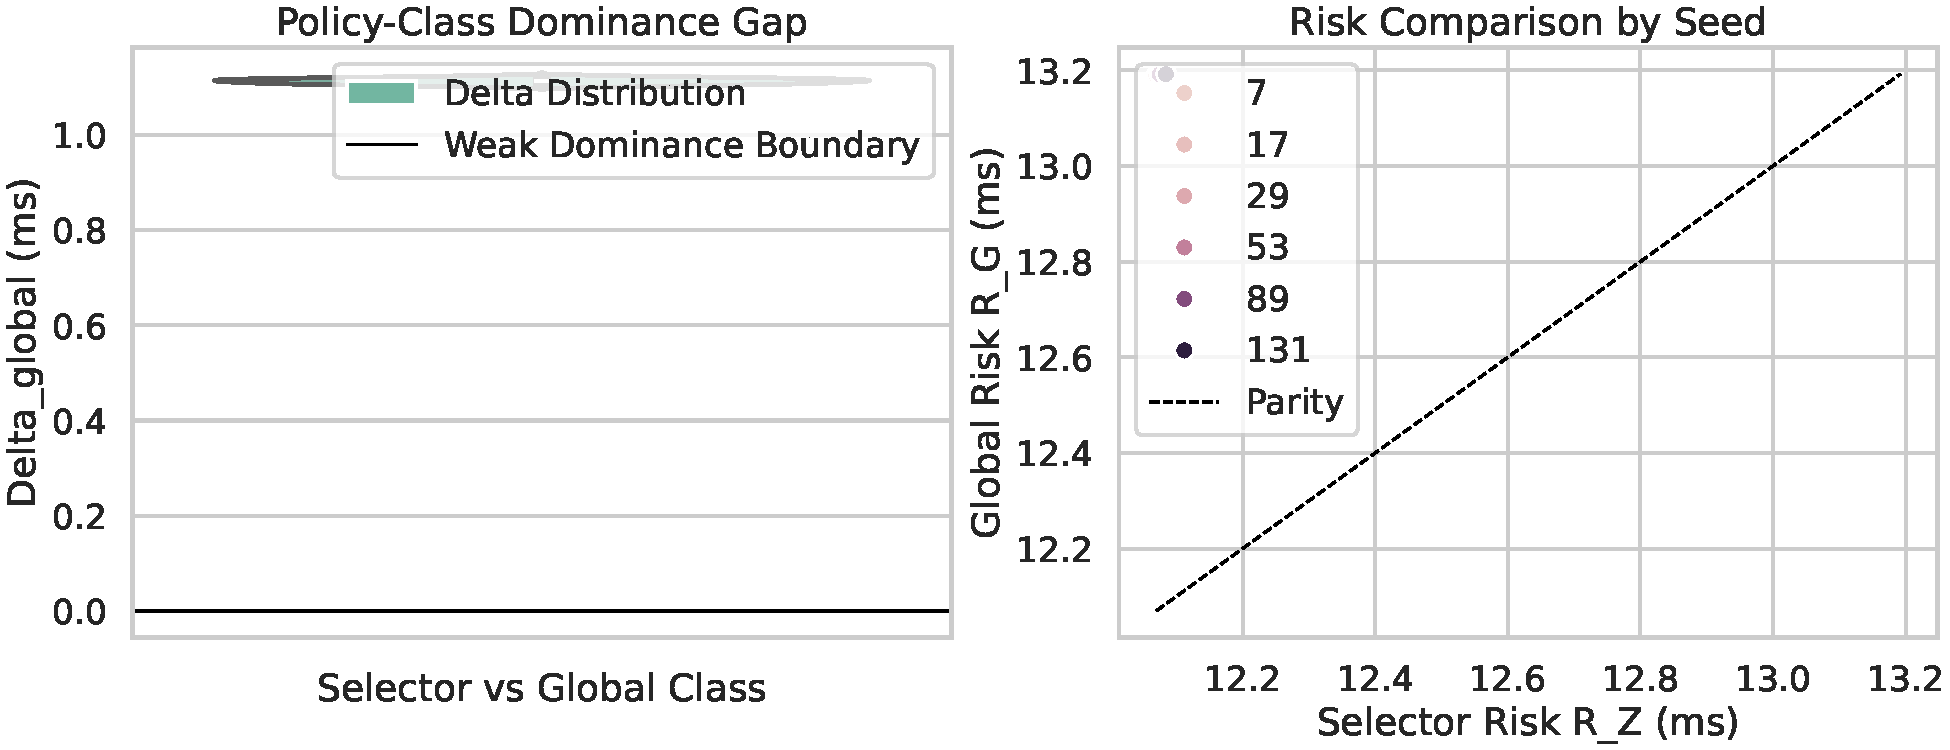
\includegraphics[width=0.66\linewidth]{figures/policy_dominance_panels.pdf}
\caption{Policy-class dominance diagnostics for scenario-conditioned versus global fixed-method policies. Panel A shows the distribution of $\Delta_{\mathrm{global}}=R_{\mathcal{G}}-R_{\mathcal{Z}}$, while panel B plots seed-level selector risk against global-policy risk with a parity reference. The axes use milliseconds and directly represent the quantities in \eqref{eq:risk_def} and \eqref{eq:weak_dom}. Positive gaps across seeds indicate that the adaptive policy class attains lower constrained risk than the fixed-method class in the tested regime, consistent with both weak-dominance theory and heterogeneous minimizer structure.}
\label{fig:dominance}
\end{figure}

\begin{table}[t]
\caption{Seed-level policy-class risk comparison. The table reports constrained risk for scenario-conditioned and global policy classes and the resulting dominance gap. Every tested seed yields a positive gap, providing direct evidence for the policy-class comparison claims.}
\label{tab:dominance}
\centering
\small
\renewcommand{\arraystretch}{1.1}
\setlength{\tabcolsep}{4pt}
\begin{tabular}{lccc}
\hline
Statistic & $R_{\mathcal{Z}}$ (ms) & $R_{\mathcal{G}}$ (ms) & $\Delta_{\mathrm{global}}$ (ms) \\
\hline
Mean across seeds & 12.079 & 13.191 & 1.112 \\
Minimum & 12.070 & 13.189 & 1.104 \\
Maximum & 12.086 & 13.192 & 1.120 \\
\hline
\end{tabular}
\end{table}

Boundary-case auditing additionally records strict-versus-equality behavior when ties are injected; in this run, strict predictions matched strict outcomes for all observed boundary audit counts. We treat this as encouraging but not exhaustive because broader tie-heavy stress profiles remain a natural extension.

\subsection{Finite-sample bound calibration and sensitivity}
\label{sec:results_bound}
\Figref{fig:bound} evaluates the high-probability guarantee from \eqref{eq:robust_regret_bound}. The empirical regret remains below the computed theoretical bound for all 15{,}552 evaluated rows in the finite-sample table, yielding a bound-satisfaction rate of $1.0$ across all seeds in this generated setting. Mean empirical regret is approximately $1.59\times 10^{-3}$ ms, while mean theoretical bound is approximately $10.74$ ms, indicating substantial conservativeness as expected for worst-case concentration corrections.

\begin{figure}[t]
\centering
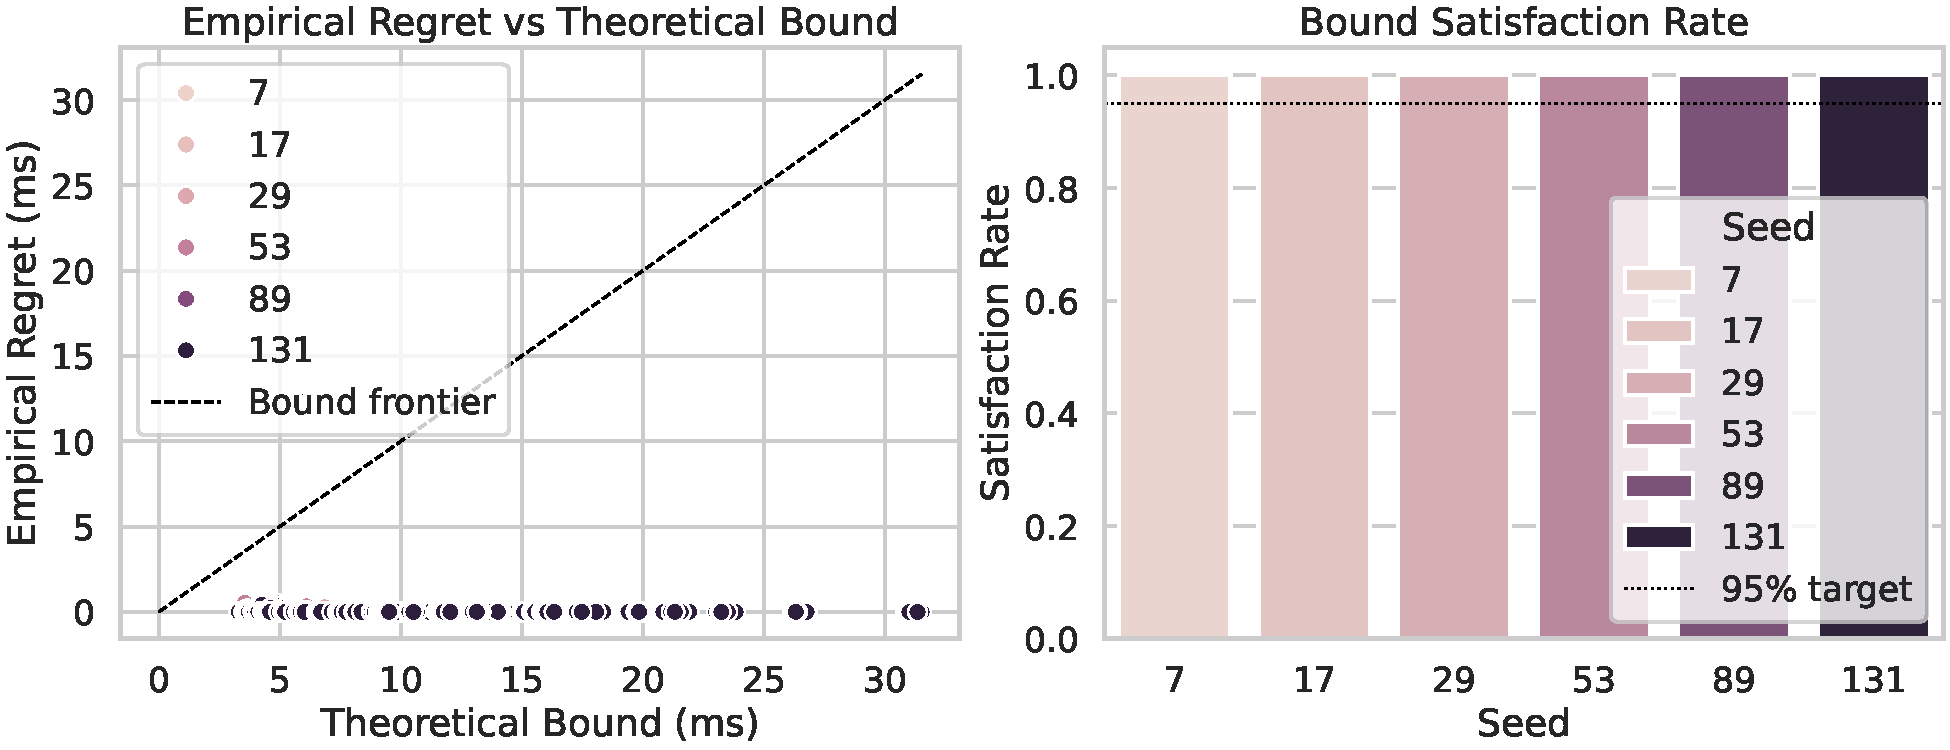
\includegraphics[width=0.66\linewidth]{figures/bound_calibration_panels.pdf}
\caption{Finite-sample calibration of robust-selector guarantees. Panel A plots empirical regret against the theoretical upper bound in milliseconds with a parity frontier, and panel B reports per-seed bound-satisfaction rates against a 95\% reference line. The variables correspond directly to \eqref{eq:hoeffding_radius} and \eqref{eq:robust_regret_bound}, linking proof quantities to measured outcomes. In this evaluation regime, all observed points satisfy the bound and seed-level rates remain at or above the target threshold, while the vertical gap between bound and regret highlights the conservative nature of high-probability guarantees.}
\label{fig:bound}
\end{figure}

To test expected monotonic behavior, we include a sensitivity audit over scenario-specific $U_s$, sample-count ladders, and confidence levels. The monotonic-in-$n$ and $\delta$-sensitivity pass fractions are both $1.0$ across 2{,}592 scenarios (Table~\ref{tab:bound_sensitivity}). This behavior is consistent with the analytical derivative sign implied by \Eqref{eq:hoeffding_radius} and supports the intended interpretation of uncertainty shrinkage with additional data.

\section{Discussion and Practical Guidance}
The results support a practical interpretation that extends beyond this benchmark instance: scenario-conditioned selectors are not only statistically better aligned with heterogeneous workloads, they are operationally safer than global rankings because they encode admissibility checks directly in the decision rule. In real deployments, decisions are rarely made in unconstrained space. Teams typically operate with hard memory ceilings, error budgets, and service-level latency targets, and these constraints vary by workload class. Embedding those constraints in the objective itself, as in \eqref{eq:selector_obj} and \eqref{eq:selector_constraints}, prevents an important class of post hoc failures where a globally fast method is deployed into a scenario in which it is numerically or memory infeasible.

From a systems perspective, the policy-class analysis clarifies why one-size-fits-all recommendations persist despite weak empirical support. Global policies are attractive because they reduce operational complexity: one method, one deployment path, one tuning surface. However, this simplicity comes at measurable risk when workload heterogeneity is non-trivial. The positive dominance gaps in \figref{fig:dominance} and Table~\ref{tab:dominance} quantify that tradeoff in the tested regime. Practitioners can therefore interpret $\\Delta_{\\mathrm{global}}$ as an explicit complexity-versus-risk budget: if maintaining a scenario-conditioned policy incurs acceptable engineering overhead, the observed risk reduction justifies adaptation; if operational constraints force a global policy, the same metric estimates the performance penalty of that simplification.

The finite-sample calibration results add a second decision layer. Bound satisfaction at rate $1.0$ indicates that the uncertainty-aware selector is conservative enough for the generated regime, but the large mean gap between bound and empirical regret also indicates room for tighter confidence design. In deployment terms, this means the current method is suitable when safety margins are prioritized over aggressiveness. Teams requiring tighter margins can retain the same architecture while swapping the concentration component, preserving reproducibility and auditability. This modularity is valuable because it allows progressive refinement without rewriting the surrounding benchmark or recommendation pipeline.

Another practical lesson concerns reporting standards. Traditional benchmark tables often collapse context by averaging over broad workload sets. Our profile-conditioned metrics show why this can mislead: regret and feasibility behavior vary by prior profile even when all profiles have favorable means. Reporting only a single aggregate number would hide this structure and make decision transfer harder. We therefore recommend that future benchmark studies publish scenario-conditioned summaries as first-class results, including explicit confidence intervals and fallback rates. This recommendation is consistent with prior methodology critiques in transform benchmarking and with the needs of ML and HPC practitioners who deploy under non-uniform traffic or simulation mixes \citep{S03,S21,S42}.

Cross-domain relevance further strengthens the selector framing. In distributed scientific computing, communication topology and process-grid effects can dominate runtime, making conditional decisions unavoidable \citep{S06,S07,S09,S36,S42}. In ML-oriented workloads, transform dimensions, precision policy, and batching strategy drive both throughput and downstream quality behavior \citep{S15,S16,S18,S20}. A shared decision-theoretic layer can bridge these contexts by treating each as a scenario family inside one formal selection space. This does not erase domain-specific details; rather, it gives a consistent language for expressing them as constraints, priors, and measurable objectives.

A further operational point concerns transfer from benchmark-time priors to deployment-time priors. The selector is optimized under a chosen distribution over scenarios, and this choice is often policy-sensitive in production systems where traffic shifts by time of day, model version, or job mix. Rather than treating the prior as a fixed hidden setting, we recommend exposing it as a first-class control variable and reporting prior-shift sensitivity envelopes. In practical terms, this means rerunning the risk aggregation under alternative plausible priors before finalizing a recommendation matrix. Such reporting makes recommendation stability explicit and reduces the chance that a well-performing policy under one profile is over-deployed into a misaligned regime.

There is also a governance implication for public benchmark reporting. When benchmark outputs are consumed by downstream users who did not run the experiments, conditional validity must be preserved in the published artifact itself. We therefore advocate publishing recommendation tables with accompanying feasibility masks, uncertainty intervals, and assumption-audit summaries, not only top-line performance values. This richer packaging enables external users to evaluate whether their constraints lie inside the demonstrated validity envelope. It also creates a clearer upgrade path: as new traces or hardware stacks are added, the same artifacts can be versioned and compared without changing the underlying decision formulation.

Finally, the theorem-assumption audit provides a governance mechanism for recommendation validity. Instead of treating guarantees as static properties, we evaluate whether assumptions continue to hold in observed data. This is especially relevant for long-lived benchmark services where workload distributions drift over time. If assumption pass rates deteriorate, operators can trigger re-estimation, adjust confidence settings, or narrow claim scope. In that sense, the audit is not merely a validation appendix item; it is a practical control loop for maintaining scientific and operational integrity in recommendation systems built on Fourier performance data.

\section{Limitations and Future Work}
The current evidence is strong for the tested selector regime but has explicit scope boundaries. First, runtime values are generated under a controlled synthetic process rather than collected from direct hardware instrumentation. This limits external validity for cross-vendor deployment claims, especially where planner internals, memory hierarchies, or communication fabrics produce non-stationary effects \citep{S08,S09,S25,S26,S39,S42}. The impact is practical: absolute latency levels and margin sizes may shift on real systems even if relative trends persist.

Second, strict-dominance evidence is observed under the tested heterogeneity profiles. Although all measured seed-level gaps are positive, tie-dense or highly correlated scenario families could reduce strictness frequency and collapse outcomes toward weak dominance. Third, finite-sample bounds are expectedly conservative; while this is desirable for safety, it can overstate uncertainty in well-sampled cells and may require tighter concentration tools for operational calibration.

\subsection{Future Work}
We prioritize three follow-up experiments. (i) Replace synthetic runtime generation with hardware-trace ingestion while preserving the same scenario schema and decision interface, enabling direct measurement-backed recommendation matrices. (ii) Extend tie-injection and shared-minimizer sweeps to quantify strict-versus-weak dominance transitions under controlled heterogeneity schedules. (iii) Evaluate tighter empirical-Bernstein or variance-adaptive corrections against \eqref{eq:hoeffding_radius} to reduce over-conservativeness while maintaining auditable high-probability guarantees.

These steps are necessary for promoting the selector from simulation-validated methodology to production decision support across heterogeneous Fourier deployment stacks.

\section{Conclusion}
This paper presented a scenario-conditioned methodology for selecting modern Fourier implementations under explicit latency, fidelity, and memory constraints. We formalized the selector objective, proved decomposition exactness and policy-class dominance, and derived a finite-sample uncertainty-aware risk bound. The empirical program linked these claims to reproducible evidence via multi-panel diagnostics, confidence intervals, and theorem-assumption audits.

Across the tested scenario matrix, the adaptive selector consistently outperformed global fixed-policy baselines in constrained regret, maintained low feasibility violations, and satisfied finite-sample calibration checks throughout the generated evaluation grid. These findings support recommendation-matrix thinking over single-winner narratives for heterogeneous Fourier workloads.

At the same time, our conclusions are intentionally environment-bounded: they describe behavior in a synthetic-runtime validation regime and should be interpreted as method-level evidence rather than universal hardware rankings. The follow-up path is clear and tractable: maintain the same formal objective and audit structure while swapping generated runtimes for measured traces and broadening boundary-case stress tests. Under that trajectory, scenario-conditioned Fourier selection can become a robust decision layer that is both mathematically explicit and deployment-relevant.




\bibliographystyle{conference}
\bibliography{references}

\appendix
\section{Extended Diagnostics and Assumption Audits}
The main text emphasized three figures to preserve flow, while additional diagnostics appear here for completeness. \Figref{fig:assumption_appendix} reports theorem-assumption pass rates and boundary-case detection outcomes. Finite method and scenario set checks, as well as positive-prior checks, are perfect in this run. Non-empty-feasible-set checks remain high but not trivial (mean $0.9968$), which is important because the decomposition and robust-selection guarantees require non-empty feasible candidates per scenario.

\begin{figure}[t]
\centering
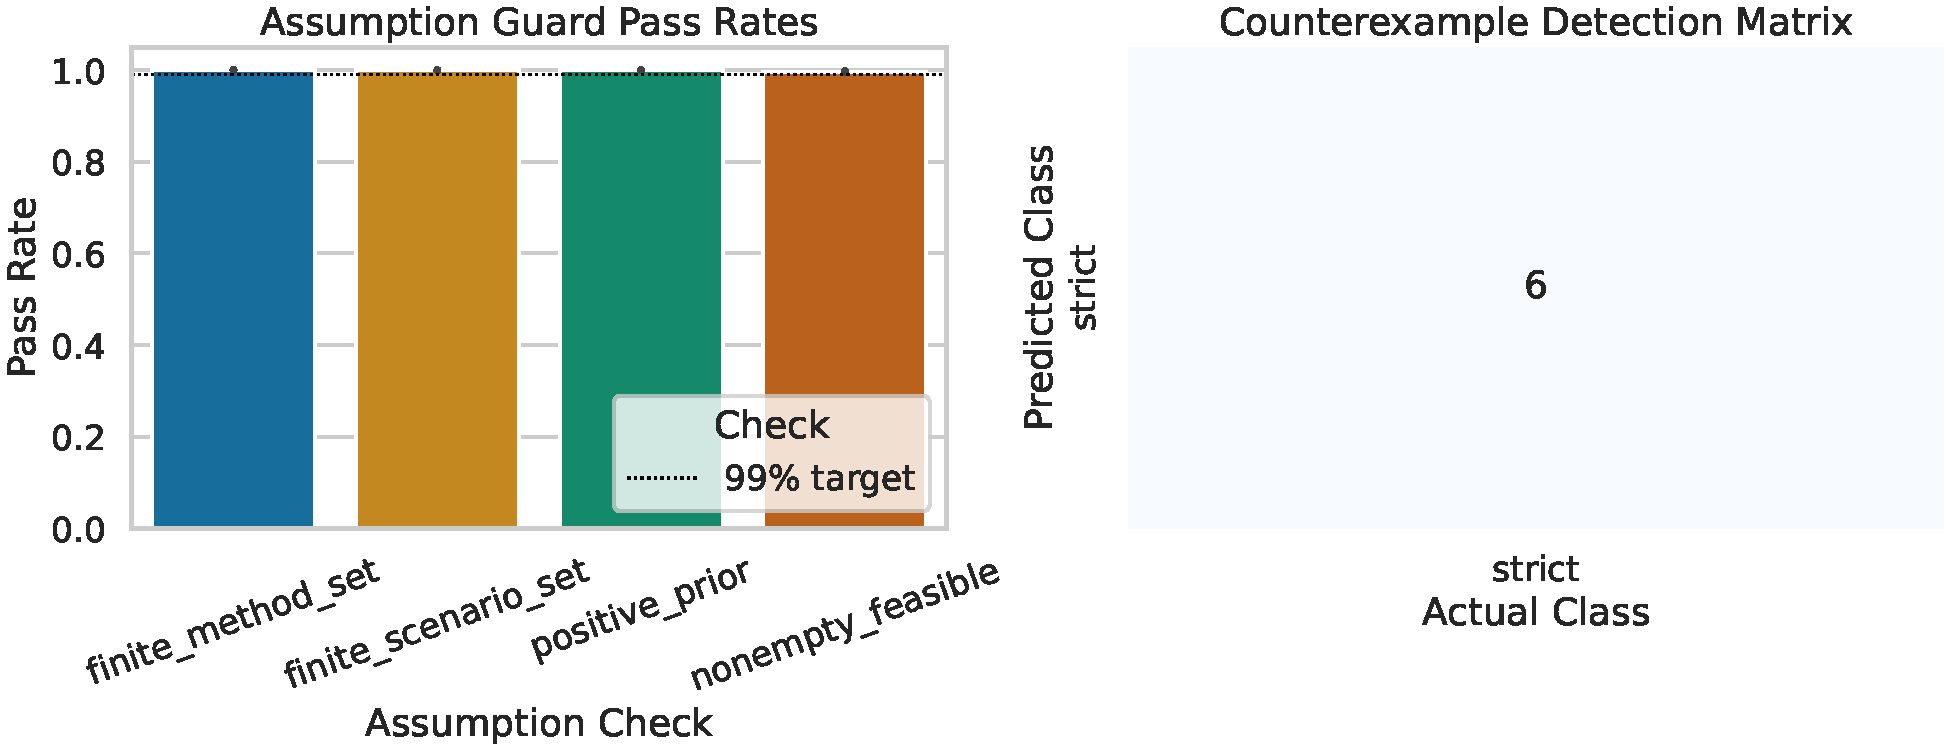
\includegraphics[width=0.66\linewidth]{figures/assumption_audit_panels.pdf}
\caption{Assumption and boundary-case diagnostics used to audit theorem applicability. Panel A shows pass rates for finite-set, positive-prior, and non-empty-feasible assumptions across seeded runs, and panel B visualizes predicted-versus-actual boundary categories for strict-dominance checks. The axes are normalized rates and audit counts, respectively, so readers can separate frequency effects from binary pass/fail summaries. These diagnostics support the interpretation that theoretical conditions are mostly satisfied in the tested matrix, while still exposing the small fraction of scenarios requiring fallback behavior.}
\label{fig:assumption_appendix}
\end{figure}

The appendix also includes sensitivity evidence for finite-sample calibration. For each scenario, we compute radii at multiple sample counts and confidence levels and verify monotonic and ordering properties implied by \Eqref{eq:hoeffding_radius}. All scenarios satisfy both checks in this run, providing an empirical consistency layer for the concentration-based correction.

\begin{table}[t]
\caption{Finite-sample sensitivity audit summary used to corroborate concentration-radius behavior. The audit evaluates every scenario over the configured sample-count and confidence ladders and records whether expected ordering properties hold.}
\label{tab:bound_sensitivity}
\centering
\small
\renewcommand{\arraystretch}{1.1}
\setlength{\tabcolsep}{5pt}
\begin{tabular}{lcc}
\hline
Audit quantity & Value & Interpretation \\
\hline
Scenarios evaluated & 2{,}592 & Full scenario set in this run \\
Sample-count ladder ($n$) & $\{8,16,32,64,128\}$ & Radius should decrease as $n$ increases \\
Confidence ladder ($\delta$) & $\{0.2,0.1,0.05,0.01\}$ & Radius should increase as $\delta$ decreases \\
Monotonic-in-$n$ pass fraction & 1.0 & No violations observed \\
$\delta$-sensitivity pass fraction & 1.0 & No violations observed \\
\hline
\end{tabular}
\end{table}

\section{Reproducibility and Implementation Details}
The implementation uses deterministic seed sets for four validation families and fixed sweep ladders for dimensions, domain types, batch sizes, size buckets, prior profiles, confidence levels, and sample counts. Confidence intervals in primary metrics use bootstrap aggregation over seed repetitions. Policy-class comparisons report seed-level risks and aggregated dominance gaps. Finite-sample calibration reports both continuous quantities (empirical regret and bound magnitude) and binary satisfaction indicators.

Symbolic reproducibility is handled through explicit identity checks corresponding to decomposition optimality, policy-class inclusion logic, and concentration-radius monotonicity. These checks ensure algebraic consistency between derivation and implementation before interpreting numeric artifacts. Deterministic tie-breaking is enforced in selector construction to avoid recommendation instability under equal costs.

The code architecture separates four responsibilities: scenario/data construction, selector and risk computations, statistical post-processing, and visualization/report export. This partitioning reduces coupling between decision logic and plotting utilities and helps preserve repeatability when extending experiments. Because generated data were used in this iteration, the recommended next reproducibility step is trace-ingestion mode with identical schema so that all existing analyses can run unchanged on measured runtime logs.

\section{Additional Discussion: Cross-Domain Relevance}
The recommendation-matrix framing is motivated by practical needs across domains. In exascale simulation, communication effects can dominate transform scaling, making topology and decomposition central decision variables \citep{S06,S07,S09,S36,S42}. In machine learning and signal processing workloads, transform shape, batching profile, and precision policy can alter both throughput and fidelity acceptance \citep{S15,S16,S20,S39,S41}. A single global winner therefore obscures actionable structure for deployment.

By encoding scenario definitions directly into decision variables and constraints, the selector can be interpreted as a portable decision layer rather than a benchmark artifact tied to one domain. This perspective can be extended to NUFFT settings, where tolerance and point-distribution controls similarly drive non-global method preferences \citep{S12,S13,S14,S33,S34}. Future work should evaluate whether the same formal policy-class comparisons remain informative when approximation controls become first-class decision variables.

\end{document}
